%-----------------------------------
% Define document and include general packages
%-----------------------------------
% Tabellen- und Abbildungsverzeichnis stehen normalerweise nicht im
% Inhaltsverzeichnis. Gleiches gilt für das Abkürzungsverzeichnis (siehe unten).
% Manche Dozenten bemängeln das. Die Optionen 'listof=totoc,bibliography=totoc'
% geben das Tabellen- und Abbildungsverzeichnis im Inhaltsverzeichnis (toc=Table
% of Content) aus.
% Da es aber verschiedene Regelungen je nach Dozent geben kann, werden hier
% beide Varianten dargestellt.
\documentclass[12pt,oneside,titlepage,listof=totoc,bibliography=totoc]{scrartcl}
%\documentclass[12pt,oneside,titlepage]{scrartcl}

%-----------------------------------
% Dokumentensprache
%-----------------------------------
\def\FOMEN{}% Auskommentieren um die Dokumentensprache auf englisch zu ändern
\newif\ifde
\newif\ifen

%-----------------------------------
% Meta informationen
%-----------------------------------
%-----------------------------------
% Meta Informationen zur Arbeit
%-----------------------------------

% Autor
\newcommand{\myAutor}{Luis Pflamminger}

% Titel der Arbeit
\newcommand{\myTitel}{Sign in with Google - Opportunities and risks of using single sign-on providers for managing user accounts on websites}

% Betreuer
\newcommand{\myBetreuer}{Prof. Dr. Carolin Tewes}

% Lehrveranstaltung
\newcommand{\myLehrveranstaltung}{Web \& Social Media Analytics}

% Matrikelnummer
\newcommand{\myMatrikelNr}{538276}

% Ort
\newcommand{\myOrt}{Düsseldorf}

% Datum der Abgabe
\newcommand{\myAbgabeDatum}{22. August 2022}

% Anzahl an Wörtern
\newcommand{\myWordCount}{4377}

% Semesterzahl
\newcommand{\mySemesterZahl}{6}

% Name der Hochschule
\newcommand{\myHochschulName}{FOM Hochschule für Oekonomie \& Management}

% Standort der Hochschule
\newcommand{\myHochschulStandort}{Düsseldorf}

% Studiengang
\newcommand{\myStudiengang}{Wirtschaftsinformatik (B. Sc.)}

% Art der Arbeit
\newcommand{\myThesisArt}{Project Paper}

% Zu erlangender akademische Grad
\newcommand{\myAkademischerGrad}{Bachelor of Science (B.Sc.)}

% Firma
\newcommand{\myFirma}{Deutsche Telekom AG}


\ifdefined\FOMEN
%Englisch
\entrue
\usepackage[english]{babel}
\else
%Deutsch
\detrue
\usepackage[ngerman]{babel}
\fi


\newcommand{\langde}[1]{%
   \ifde\selectlanguage{ngerman}#1\fi}
\newcommand{\langen}[1]{%
   \ifen\selectlanguage{english}#1\fi}
\usepackage[utf8]{luainputenc}
\langde{\usepackage[babel,german=quotes]{csquotes}}
\langen{\usepackage[babel,english=british]{csquotes}}
\usepackage[T1]{fontenc}
\usepackage{fancyhdr}
\usepackage{fancybox}
\usepackage[a4paper, left=4cm, right=2cm, top=4cm, bottom=2cm]{geometry}
\usepackage{graphicx}
\usepackage{subfig}
\usepackage{wrapfig}
\usepackage{colortbl}
\usepackage[capposition=top]{floatrow}
\usepackage{array}
\usepackage{float}      %Positionierung von Abb. und Tabellen mit [H] erzwingen
\usepackage{footnote}
% Darstellung der Beschriftung von Tabellen und Abbildungen (Leitfaden S. 44)
% singlelinecheck=false: macht die Caption linksbündig (statt zentriert)
% labelfont auf fett: (Tabelle x.y:, Abbildung: x.y)
% font auf fett: eigentliche Bezeichnung der Abbildung oder Tabelle
% Fettschrift laut Leitfaden 2018 S. 45
\usepackage[singlelinecheck=false, labelfont=bf, font=bf]{caption}
\usepackage{caption}
\usepackage{enumitem}
\usepackage{amssymb}
\usepackage{mathptmx}
%\usepackage{minted} %Kann für schöneres Syntax Highlighting genutzt werden. ACHTUNG: Python muss installiert sein.
\usepackage[scaled=0.9]{helvet} % Behebt, zusammen mit Package courier, pixelige Überschriften. Ist, zusammen mit mathptx, dem times-Package vorzuziehen. Details: https://latex-kurs.de/fragen/schriftarten/Times_New_Roman.html
\usepackage{courier}
\usepackage{amsmath}
\usepackage[table]{xcolor}
\usepackage{marvosym}			% Verwendung von Symbolen, z.B. perfektes Eurozeichen

\renewcommand\familydefault{\sfdefault}
\usepackage{ragged2e}

% Mehrere Fussnoten nacheinander mit Komma separiert
\usepackage[hang,multiple]{footmisc}
\setlength{\footnotemargin}{1em}

% todo Aufgaben als Kommentare verfassen für verschiedene Editoren
\usepackage{todonotes}

% Verhindert, dass nur eine Zeile auf der nächsten Seite steht
\setlength{\marginparwidth}{2cm}
\usepackage[all]{nowidow}

%-----------------------------------
% Farbdefinitionen
%-----------------------------------
\definecolor{darkblack}{rgb}{0,0,0}
\definecolor{dunkelgrau}{rgb}{0.8,0.8,0.8}
\definecolor{hellgrau}{rgb}{0.0,0.7,0.99}
\definecolor{mauve}{rgb}{0.58,0,0.82}
\definecolor{dkgreen}{rgb}{0,0.6,0}

%-----------------------------------
% Pakete für Tabellen
%-----------------------------------
\usepackage{epstopdf}
\usepackage{nicefrac} % Brüche
\usepackage{multirow}
\usepackage{rotating} % vertikal schreiben
\usepackage{mdwlist}
\usepackage{tabularx}% für Breitenangabe#
\usepackage{booktabs}

%-----------------------------------
% sauber formatierter Quelltext
%-----------------------------------
\usepackage{listings}
% JavaScript als Sprache definieren:
\lstdefinelanguage{JavaScript}{
	keywords={break, super, case, extends, switch, catch, finally, for, const, function, try, continue, if, typeof, debugger, var, default, in, void, delete, instanceof, while, do, new, with, else, return, yield, enum, let, await},
	keywordstyle=\color{blue}\bfseries,
	ndkeywords={class, export, boolean, throw, implements, import, this, interface, package, private, protected, public, static},
	ndkeywordstyle=\color{darkgray}\bfseries,
	identifierstyle=\color{black},
	sensitive=false,
	comment=[l]{//},
	morecomment=[s]{/*}{*/},
	commentstyle=\color{purple}\ttfamily,
	stringstyle=\color{red}\ttfamily,
	morestring=[b]',
	morestring=[b]"
}

\lstset{
	%language=JavaScript,
	numbers=left,
	numberstyle=\tiny,
	numbersep=5pt,
	breaklines=true,
	showstringspaces=false,
	frame=single ,
	xleftmargin=5pt,
	xrightmargin=5pt,
	basicstyle=\ttfamily\scriptsize,
	stepnumber=1,
	keywordstyle=\color{blue},          % keyword style
  	commentstyle=\color{dkgreen},       % comment style
  	stringstyle=\color{mauve}         % string literal style
}

%-----------------------------------
%Literaturverzeichnis Einstellungen
%-----------------------------------

% Biblatex

\usepackage{url}
\urlstyle{same}

%%%% Neuer Leitfaden (2018)
\usepackage[
backend=biber,
%style=ieee,
style=ext-authoryear-ibid,
maxcitenames=3,	% mindestens 3 Namen ausgeben bevor et. al. kommt
maxbibnames=999,
mergedate=false,
date=iso,
seconds=true, %werden nicht verwendet, so werden aber Warnungen unterdrückt.
urldate=iso,
innamebeforetitle,
dashed=false,
autocite=footnote,
useprefix=true, % 'von' im Namen beachten (beim Anzeigen)
mincrossrefs = 1
]{biblatex}%iso dateformat für YYYY-MM-DD

%weitere Anpassungen für BibLaTex
\usepackage{xpatch}

\setlength\bibhang{1cm}

%%% Weitere Optionen
%\boolitem[false]{citexref} %Wenn incollection, inbook, inproceedings genutzt wird nicht den zugehörigen parent auch in Literaturverzeichnis aufnehmen

%Aufräumen die Felder werden laut Leitfaden nicht benötigt.
\AtEveryBibitem{%
\ifentrytype{book}{
    \clearfield{issn}%
    \clearfield{doi}%
    \clearfield{isbn}%
    \clearfield{url}
    \clearfield{eprint}
}{}
\ifentrytype{collection}{
  \clearfield{issn}%
  \clearfield{doi}%
  \clearfield{isbn}%
  \clearfield{url}
  \clearfield{eprint}
}{}
\ifentrytype{incollection}{
  \clearfield{issn}%
  \clearfield{doi}%
  \clearfield{isbn}%
  \clearfield{url}
  \clearfield{eprint}
}{}
\ifentrytype{article}{
  \clearfield{issn}%
  \clearfield{doi}%
  \clearfield{isbn}%
  \clearfield{url}
  \clearfield{eprint}
}{}
\ifentrytype{inproceedings}{
  \clearfield{issn}%
  \clearfield{doi}%
  \clearfield{isbn}%
  \clearfield{url}
  \clearfield{eprint}
}{}
}
\renewcommand*{\finentrypunct}{}%Kein Punkt am ende des Literaturverzeichnisses

\renewcommand*{\newunitpunct}{\addcomma\space}
\DeclareDelimFormat[bib,biblist]{nametitledelim}{\addcolon\space}
\DeclareDelimFormat{titleyeardelim}{\newunitpunct}
%Namen kursiv schreiben
\renewcommand*{\mkbibnamefamily}{\mkbibemph}
\renewcommand*{\mkbibnamegiven}{\mkbibemph}
\renewcommand*{\mkbibnamesuffix}{\mkbibemph}
\renewcommand*{\mkbibnameprefix}{\mkbibemph}

% Die Trennung mehrerer Autorennamen erfolgt durch Kommata.
% siehe Beispiele im Leitfaden S. 16
% Die folgende Zeile würde mit Semikolon trennen
%\DeclareDelimFormat{multinamedelim}{\addsemicolon\addspace}

%Delimiter für mehrere und letzten Namen gleich setzen
\DeclareDelimAlias{finalnamedelim}{multinamedelim}

\DeclareNameAlias{default}{family-given}
\DeclareNameAlias{sortname}{default}  %Nach Namen sortieren


\DeclareFieldFormat{editortype}{\mkbibparens{#1}}
\DeclareDelimFormat{editortypedelim}{\addspace}
\DeclareFieldFormat{translatortype}{\mkbibparens{#1}}
\DeclareDelimFormat{translatortypedelim}{\addspace}
\DeclareDelimFormat[bib,biblist]{innametitledelim}{\addcomma\space}

\DeclareFieldFormat*{citetitle}{#1}
\DeclareFieldFormat*{title}{#1}
\DeclareFieldFormat*{booktitle}{#1}
\DeclareFieldFormat*{journaltitle}{#1}

\xpatchbibdriver{online}
  {\usebibmacro{organization+location+date}\newunit\newblock}
  {}
  {}{}
\DeclareFieldFormat[online]{date}{\mkbibparens{#1}}
\DeclareFieldFormat{urltime}{\addspace #1\addspace \langde{Uhr}\langen{MEZ}}
\DeclareFieldFormat{urldate}{%urltime zu urldate hinzufügen
  [\langde{Zugriff}\langen{Access}\addcolon\addspace
  #1\printfield{urltime}]
}
\DeclareFieldFormat[online]{url}{<\url{#1}>}
\renewbibmacro*{url+urldate}{%
  \usebibmacro{url}%
  \ifentrytype{online}
    {\setunit*{\addspace}%
     \iffieldundef{year}
       {\printtext[date]{\langde{keine Datumsangabe}\langen{no Date}}}
       {\usebibmacro{date}}}%
    {}%
  \setunit*{\addspace}%
  \usebibmacro{urldate}
  }

%Verhindern, dass bei mehreren Quellen des gleichen Autors im gleichen Jahr
%Buchstaben nach der Jahreszahl angezeigt werden wenn sich das Keyword in usera unterscheidet.
\DeclareExtradate{
  \scope{
    \field{labelyear}
    \field{year}
    }
    \scope{
      \field{usera}
     }
}

%% Anzeige des Jahres nach dem Stichwort (usera) im Literaturverzeichnis
%% Wenn das Jahr bei Online-Quellen nicht explizit angegeben wurde, wird nach
%% dem Stichwort 'o. J.' ausgegeben. Nach der URL steht dann 'keine
%% Datumsangabe'. Ist das Jahr definiert, wird es an beiden Stellen ausgegeben.
%% Das Zugriffsdatum (urldate) spielt hier keine Rolle.
%% Für Nicht-Online-Quellen wird nichts geändert.
\renewbibmacro*{date+extradate}{%
  \printtext[parens]{%
    \printfield{usera}%
    \setunit{\printdelim{titleyeardelim}}%
    \ifentrytype{online}
       {\setunit*{\addspace\addcomma\addspace}%
         \iffieldundef{year}
           {\bibstring{nodate}}
       {\printlabeldateextra}}%
       {\printlabeldateextra}}}

% Anzeige des Jahres nach dem Stichwort (usera) in der Fussnote
% das Stichwort hat der Aufrufer hier schon ausgegeben.
% siehe auch Kommentar zu: \renewbibmacro*{date+extradate}
\renewbibmacro*{cite:labeldate+extradate}{%
    \ifentrytype{online}
       {\setunit*{\addspace\addcomma\addspace}%
         \iffieldundef{year}
           {\bibstring{nodate}}
       {\printlabeldateextra}}%
       {\printlabeldateextra}}
\DefineBibliographyStrings{german}{
  nodate    = {{}o.\adddot\addspace J\adddot},
  andothers = {et\addabbrvspace al\adddot}
}
\DefineBibliographyStrings{english}{
  nodate    = {{}n.\adddot\addspace d\adddot},
  andothers = {et\addabbrvspace al\adddot}
}
%%% PROBLEMSTELLE
\DeclareSourcemap{
  \maps[datatype=bibtex]{
    \map{
      \step[notfield=translator, final]
      \step[notfield=editor, final]
      %\step[fieldset=author, fieldvalue={{{\langde{o\noexpand\adddot\addspace V\noexpand\adddot}\langen{Anon}}}}]
      \step[fieldset=author, fieldvalue={Anon}]
    }
    \map{
      \pernottype{online}
      \step[fieldset=location, fieldvalue={\langde{o\noexpand\adddot\addspace O\noexpand\adddot}\langen{s\noexpand\adddot I\noexpand\adddot}}]
    }
  }
}

\renewbibmacro*{cite}{%
  \iffieldundef{shorthand}
    {\ifthenelse{\ifnameundef{labelname}\OR\iffieldundef{labelyear}}
       {\usebibmacro{cite:label}%
        \setunit{\printdelim{nonametitledelim}}}
       {\printnames{labelname}%
        \setunit{\printdelim{nametitledelim}}}%
     \printfield{usera}%
     \setunit{\printdelim{titleyeardelim}}%
     \usebibmacro{cite:labeldate+extradate}}
    {\usebibmacro{cite:shorthand}}}

    \renewcommand*{\jourvoldelim}{\addcomma\addspace}% Trennung zwischen journalname und Volume. Sonst Space; Laut Leitfaden richtig
  %Aufgrund der Änderung bzgl des Issues 169 in der thesis_main.tex musste ich die Zeile auskommentieren. Konnte aber das Verhalten, dass die Fußnoten grün sind, im nachhinein nicht feststellen.
  %\hypersetup{hidelinks} %sonst sind Fußnoten grün. Dadurch werden Links allerdings nicht mehr farbig dargestellt
\renewbibmacro*{journal+issuetitle}{%
  \usebibmacro{journal}%
  \setunit*{\jourvoldelim}%
  \iffieldundef{series}
    {}
    {\setunit*{\jourserdelim}%
     \printfield{series}%
     \setunit{\servoldelim}}%
  \iffieldundef{volume}
    {}
    {\printfield{volume}}
  \iffieldundef{labelyear}
  {}
  {
  (\thefield{year}) %Ansonsten wird wenn kein Volume angegeben ist ein Komma vorangestellt
  }
  \setunit*{\addcomma\addspace Nr\adddot\addspace}
  \printfield{number}
  \iffieldundef{eid}
  {}
  {\printfield{eid}}
}

% Postnote ist der Text in der zweiten eckigen Klammer bei einem Zitat
% wenn es keinen solchen Eintrag gibt, dann auch nicht ausgeben, z.B. 'o. S.'
% Wenn man das will, kann man das 'o. S.' ja explizit angeben. Andernfalls steht
% sonst auch bei Webseiten 'o. S.' da, was laut Leitfaden nicht ok ist.
\renewbibmacro*{postnote}{%
  \setunit{\postnotedelim}%
  \iffieldundef{postnote}
    {} %{\printtext{\langde{o.S\adddot}\langen{no page number}}}
    {\printfield{postnote}}}

% Abstand bei Änderung Anfangsbuchstabe ca. 1.5 Zeilen
\setlength{\bibinitsep}{0.75cm}

% nur in den Zitaten/Fussnoten den Vornamen abkürzen (nicht im
% Literaturverzeichnis)

\DeclareDelimFormat{nonameyeardelim}{\addcomma\space}
\DeclareDelimFormat{nameyeardelim}{\addcomma\space}

\renewbibmacro*{cite}{%
  \iffieldundef{shorthand}
    {\ifthenelse{\ifciteibid\AND\NOT\iffirstonpage}
       {\usebibmacro{cite:ibid}}
    {\printtext[bibhyperref]{\ifthenelse{\ifnameundef{labelname}\OR\iffieldundef{labelyear}}
       {\usebibmacro{cite:label}%
        \setunit{\printdelim{nonameyeardelim}}}
      {\toggletrue{abx@bool@giveninits}%
        \printnames[family-given]{labelname}%
        \setunit{\printdelim{nameyeardelim}}}%
      \printfield{usera}%
      \setunit{\printdelim{titleyeardelim}}%
     \usebibmacro{cite:labeldate+extradate}}}}
   {\usebibmacro{cite:shorthand}}}


%%%%% Alter Leitfaden. Ggf. Einkommentieren und Bereich hierüber auskommentieren
%\usepackage[
%backend=biber,
%style=numeric,
%citestyle=authoryear,
%url=false,
%isbn=false,
%notetype=footonly,
%hyperref=false,
%sortlocale=de]{biblatex}

%weitere Anpassungen für BibLaTex
%% Optionen für Biblatex
\ExecuteBibliographyOptions{%
giveninits=false,
isbn=true,
url=true,
doi=false,
eprint=false,
maxbibnames=7, % Alle Autoren (kein et al.)
maxcitenames=2, % et al. ab dem 3. Autor
backref=false, % Rückverweise auf Zitatseiten
bibencoding=utf8, % wenn .bib in utf8, sonst ascii
bibwarn=true, % Warnung bei fehlerhafter bib-Datei
}%

% et al. an Stelle von u.a.
\DefineBibliographyStrings{ngerman}{
   andothers = {{et\,al\adddot}},
}

% Klammern um das Jahr in der Fußnote
\renewbibmacro*{cite:labelyear+extrayear}{%
  \iffieldundef{labelyear}
    {}
    {\printtext[bibhyperref]{%
       \mkbibparens{%
         \printfield{labelyear}%
         \printfield{extrayear}}}}}

\renewbibmacro*{cite:title}{%
  \printtext[bibhyperref]{%
    \printfield[citetitle]{labeltitle}%
    \setunit{\addcomma\space}%
    \printdate}}

\DeclareNameFormat{last-first}{%
  \iffirstinits
    {\usebibmacro{name:family-given}
        {\namepartfamily}
        {\namepartgiveni}
        {\namepartprefix}
        {\namepartsuffix}
    }
    {\usebibmacro{name:family-given}
        {\namepartfamily}
        {\namepartgiven}
        {\namepartprefix}
        {\namepartsuffix}
    }%
  \usebibmacro{name:andothers}}

% Alternative Notation der Fußnoten
% Zeigt sowohl den Nachnamen als auch den Vornamen an
% Beispiel: \fullfootcite[Vgl. ][Seite 5]{Tanenbaum.2003}
\DeclareCiteCommand{\fullfootcite}[\mkbibfootnote]
  {\usebibmacro{prenote}}
  {\usebibmacro{citeindex}%
    \printnames[sortname][1-1]{author}%
    \addspace (\printfield{year})}
  {\addsemicolon\space}
  {\usebibmacro{postnote}}

%Autoren (Nachname, Vorname)
\DeclareNameAlias{default}{family-given}

%Reihenfolge von publisher, year, address verändern
% Achtung, bisher nur für den Typ @book definiert

%% Definiert @Book Eintrag
\DeclareBibliographyDriver{book}{%
  \printnames{author}%
  \newunit\addcolon\space
  \printfield{title}%
  \setunit*{,\space}%
  \printfield{edition}%
  \setunit*{\addcomma\space}%
  \printlist{publisher}%
  \newunit\newblockpunct
  \printlist{location}%
  \setunit*{\space}%
  \printfield{year}%
  \setunit*{,\space}%
  \printfield{isbn}%
  \finentry}

%% Definiert @Online Eintrag
\DeclareBibliographyDriver{online}{%
  \printnames{author}%
  \newunit\newblockpunct
  \printfield{title}%
  \setunit*{,\space}%
  %\newunit\newblock
  \printfield{url}%
  \setunit*{,\space Erscheinungsjahr:\space}%
  \printfield{year}%
  \setunit*{,\space Aufruf am:\space}%
  \printfield{note}%
  \finentry}

%% Definiert @Article Eintrag
\DeclareBibliographyDriver{article}{%
  \printnames{author}%
  \newunit\newblockpunct
  \printfield{title}%
  \setunit*{.\space In:\space}%
  %\newunit\newblock
  \usebibmacro{journal}%
  \setunit*{\space (}%
  \printfield{year}\newunit{)}%
  \finentry}

%% Definiert @InProceedings Eintrag
\DeclareBibliographyDriver{inproceedings}{%
	\printnames{author}%
	\setunit*{,\space (}%
	\printfield{year}\newunit{)}%
	\newunit\newblockpunct
	\printfield{title}%
	\setunit*{\space}%
	\usebibmacro{booktitle}%
	\setunit*{,\space}%
	\printfield{isbn}%
	\setunit*{,\space}%
	\printfield{doi}%
	\finentry}

%Doppelpunkt nach dem letzten Autor
\renewcommand*{\labelnamepunct}{\addcolon\addspace }

%Komma an Stelle des Punktes
\renewcommand*{\newunitpunct}{\addcomma\space}

%Autoren durch Semikolon trennen
\newcommand*{\bibmultinamedelim}{\addsemicolon\space}%
\newcommand*{\bibfinalnamedelim}{\addsemicolon\space}%
\AtBeginBibliography{%
  \let\multinamedelim\bibmultinamedelim
  \let\finalnamedelim\bibfinalnamedelim
}

%Titel nicht kursiv anzeigen
\DeclareFieldFormat{title}{#1\isdot}


%%%% Ende Alter Leitfaden

%Bib-Datei einbinden
\addbibresource{literature/literature.bib}

% Zeilenabstand im Literaturverzeichnis ist Einzeilig
% siehe Leitfaden S. 14
\AtBeginBibliography{\singlespacing}

%-----------------------------------
% Silbentrennung
%-----------------------------------
\usepackage{hyphsubst}
\HyphSubstIfExists{ngerman-x-latest}{%
\HyphSubstLet{ngerman}{ngerman-x-latest}}{}

%-----------------------------------
% Pfad fuer Abbildungen
%-----------------------------------
\graphicspath{{./}{./figures/}}

%-----------------------------------
% Weitere Ebene einfügen
%-----------------------------------
\usepackage{titletoc}

\makeatletter

% Setze die Tiefe des Inhaltsverzeichnis auf 4 Ebenen
% Damit erscheinen \paragraph-Sektionen auch im Inhaltsverzeichnis
\setcounter{secnumdepth}{4}
\setcounter{tocdepth}{4}

% Fuege Abstand nach unten wie in einer normalen \section hinzu
% Andernfalls haette \paragraph keinen Zeilenumbruch
% Der Zeilenumbruch koennte mit einer leeren \mbox{} ersetzt werden
% Jedoch klebt dann der Text relativ nah an der Ueberschrift
\renewcommand{\paragraph}{%
  \@startsection{paragraph}{4}%
  {\z@}{3.25ex \@plus 1ex \@minus .2ex}{1.5ex plus 0.2ex}%
  {\normalfont\normalsize\bfseries\sffamily}%
}

\makeatother


%-----------------------------------
% Paket für die Nutzung von Anhängen
%-----------------------------------
\usepackage{appendix}

%-----------------------------------
% Zeilenabstand 1,5-zeilig
%-----------------------------------
\usepackage{setspace}
\onehalfspacing

%-----------------------------------
% Absätze durch eine neue Zeile
%-----------------------------------
\setlength{\parindent}{0mm}
\setlength{\parskip}{0.8em plus 0.5em minus 0.3em}

\sloppy					%Abstände variieren
\pagestyle{headings}

%----------------------------------
% Präfix in das Abbildungs- und Tabellenverzeichnis aufnehmen, statt nur der Nummerierung (siehe Issue #206).
%----------------------------------
\KOMAoption{listof}{entryprefix} % Siehe KOMA-Script Doku v3.28 S.153
\BeforeStartingTOC[lof]{\renewcommand*\autodot{:}} % Für den Doppelpunkt hinter Präfix im Abbildungsverzeichnis
\BeforeStartingTOC[lot]{\renewcommand*\autodot{:}} % Für den Doppelpunkt hinter Präfix im Tabellenverzeichnis

%-----------------------------------
% Abkürzungsverzeichnis
%-----------------------------------
\usepackage[printonlyused]{acronym}

%-----------------------------------
% Symbolverzeichnis
%-----------------------------------
% Quelle: https://www.namsu.de/Extra/pakete/Listofsymbols.pdf
\usepackage[final]{listofsymbols}

%-----------------------------------
% Glossar
%-----------------------------------
%\usepackage{glossaries}
%\glstoctrue %Auskommentieren, damit das Glossar nicht im Inhaltsverzeichnis angezeigt wird.
%\makenoidxglossaries
%\input{abkuerzungen/glossar}

%-----------------------------------
% PDF Meta Daten setzen
%-----------------------------------
\usepackage[hyperfootnotes=false]{hyperref} %hyperfootnotes=false deaktiviert die Verlinkung der Fußnote. Ansonsten inkompaibel zum Paket "footmisc"
% Behebt die falsche Darstellung der Lesezeichen in PDF-Dateien, welche eine Übersetzung besitzen
% siehe Issue 149
\makeatletter
\pdfstringdefDisableCommands{\let\selectlanguage\@gobble}
\makeatother

\hypersetup{
    pdfinfo={
        Title={\myTitel},
        Subject={\myStudiengang},
        Author={\myAutor},
        Build=1.1
    }
}

%-----------------------------------
% Technical packages
%-----------------------------------
%\usepackage{plantuml}
%\usepackage{rest-api}
%\breakRoute %enables pagebreaks during api call diagrams

%-----------------------------------
% Umlaute in Code korrekt darstellen
% siehe auch: https://en.wikibooks.org/wiki/LaTeX/Source_Code_Listings
%-----------------------------------
\lstset{literate=
	{á}{{\'a}}1 {é}{{\'e}}1 {í}{{\'i}}1 {ó}{{\'o}}1 {ú}{{\'u}}1
	{Á}{{\'A}}1 {É}{{\'E}}1 {Í}{{\'I}}1 {Ó}{{\'O}}1 {Ú}{{\'U}}1
	{à}{{\`a}}1 {è}{{\`e}}1 {ì}{{\`i}}1 {ò}{{\`o}}1 {ù}{{\`u}}1
	{À}{{\`A}}1 {È}{{\'E}}1 {Ì}{{\`I}}1 {Ò}{{\`O}}1 {Ù}{{\`U}}1
	{ä}{{\"a}}1 {ë}{{\"e}}1 {ï}{{\"i}}1 {ö}{{\"o}}1 {ü}{{\"u}}1
	{Ä}{{\"A}}1 {Ë}{{\"E}}1 {Ï}{{\"I}}1 {Ö}{{\"O}}1 {Ü}{{\"U}}1
	{â}{{\^a}}1 {ê}{{\^e}}1 {î}{{\^i}}1 {ô}{{\^o}}1 {û}{{\^u}}1
	{Â}{{\^A}}1 {Ê}{{\^E}}1 {Î}{{\^I}}1 {Ô}{{\^O}}1 {Û}{{\^U}}1
	{œ}{{\oe}}1 {Œ}{{\OE}}1 {æ}{{\ae}}1 {Æ}{{\AE}}1 {ß}{{\ss}}1
	{ű}{{\H{u}}}1 {Ű}{{\H{U}}}1 {ő}{{\H{o}}}1 {Ő}{{\H{O}}}1
	{ç}{{\c c}}1 {Ç}{{\c C}}1 {ø}{{\o}}1 {å}{{\r a}}1 {Å}{{\r A}}1
	{€}{{\EUR}}1 {£}{{\pounds}}1 {„}{{\glqq{}}}1
}

%\usepackage[final]{pdfpages}
%\setboolean{@twoside}{false}

%-----------------------------------
% Kopfbereich / Header definieren
%-----------------------------------
\pagestyle{fancy}
\fancyhf{}
% Seitenzahl oben, mittig, mit Strichen beidseits
% \fancyhead[C]{-\ \thepage\ -}

% Seitenzahl oben, mittig, entsprechend Leitfaden ohne Striche beidseits
\fancyhead[C]{\thepage}
%\fancyhead[L]{\leftmark}							% kein Footer vorhanden
% Waagerechte Linie unterhalb des Kopfbereiches anzeigen. Laut Leitfaden ist
% diese Linie nicht erforderlich. Ihre Breite kann daher auf 0pt gesetzt werden.
\renewcommand{\headrulewidth}{0.4pt}
%\renewcommand{\headrulewidth}{0pt}

%-----------------------------------
% Damit die hochgestellten Zahlen auch auf die Fußnote verlinkt sind (siehe Issue 169)
%-----------------------------------
\hypersetup{colorlinks=true, breaklinks=true, linkcolor=darkblack, citecolor=darkblack, menucolor=darkblack, urlcolor=darkblack, linktoc=all, bookmarksnumbered=false, pdfpagemode=UseOutlines, pdftoolbar=true}
\urlstyle{same}%gleiche Schriftart für den Link wie für den Text

%-----------------------------------
% Start the document here:
%-----------------------------------
\begin{document}

\pagenumbering{Roman}								% Seitennumerierung auf römisch umstellen
\newcolumntype{C}{>{\centering\arraybackslash}X}	% Neuer Tabellen-Spalten-Typ:
%Zentriert und umbrechbar

%-----------------------------------
% Textcommands
%-----------------------------------
%----------------------------------
%  TextCommands
%----------------------------------
%
%
%
%
%----------------------------------
%  common textCommands
%----------------------------------
% Information: OL bedeutet ohne Leerzeichen. Damit man dieses Command z. B. vor einem Komma oder vor einem anderen Zeichen verwenden kann. Dies ist ein Best-Practis von mir und hat sich sehr bewehrt.
% Allgemein hat es sich bewert alle Wörter die man häufig schreibt und wahrscheinlich falsch oder unterscheidlich schreibt, als Textcommand zu hinterlegen.
% 
%
%
\renewcommand{\symheadingname}{\langde{Symbolverzeichnis}\langen{List of Symbols}}
\newcommand{\abbreHeadingName}{\langde{Abkürzungsverzeichnis}\langen{List of Abbreviations}}
\newcommand{\headingNameInternetSources}{\langde{Internetquellen}\langen{Internet sources}}
\newcommand{\AppendixName}{\langde{Anhang}\langen{Appendix}}
\newcommand{\vglf}{\langde{Vgl.}\langen{compare}}
\newcommand{\pagef}{\langde{S. }\langen{p. }}
\newcommand{\os}{\mbox{o. S}}
\newcommand{\ojol}{\mbox{o. J.}}
\newcommand{\oj}{\ojol\ }
\newcommand{\og}{\mbox{o. g.}\ }
\newcommand{\ua}{\mbox{u. a.}\ }
\newcommand{\dah}{\mbox{d. h.}\ }
\newcommand{\zbol}{\mbox{z. B.}}
\newcommand{\zb}{\zbol\ }
\newcommand{\uamol}{unter anderem}
\newcommand{\uam}{\uamol\ }
\newcommand{\uanol}{unter anderen}%mit Leerzeichen
\newcommand{\uan}{\uanol\ }%mit Leerzeichen
\newcommand{\abbol}{Ab"-bil"-dung}
\newcommand{\abb}{\abbol\ }
\newcommand{\tabol}{Tabelle}
\newcommand{\tab}{\tabol\ }
\newcommand{\ggfol}{ggf.}
\newcommand{\ggf}{\ggfol\ }
\newcommand{\unodol}{und/oder}
\newcommand{\unod}{\unodol\ }

%----------------------------------
% project individual textCommands
%----------------------------------
\newcommand{\lehol}{Lebensmitteleinzelhandel}%Beispiel eines langen Wortes
\newcommand{\leh}{\lehol\ }


%-----------------------------------
% Titlepage
%-----------------------------------
\begin{titlepage}
	\newgeometry{left=2cm, right=2cm, top=2cm, bottom=2cm}
	\begin{center}
    
\includegraphics[width=2.3cm]{figures/fomLogo} \\
    \vspace{.5cm}
		\begin{Large}\textbf{\myHochschulName}\end{Large}\\
    \vspace{.5cm}
		\begin{Large}\langde{Hochschulzentrum}\langen{Hochschulzentrum} \myHochschulStandort\end{Large}\\
		\vspace{1cm}
    \large{\textbf{\myThesisArt}}\\
	\langde{Berufsbegleitender Studiengang}
	\langen{part-time degree program}\\
	\mySemesterZahl . Semester\\
    \langde{im Studiengang}\langen{in the study course} \myStudiengang
		\vspace{0.5cm}

		%\langde{zur Erlangung des Grades eines}\langen{to obtain the degree of}\\
    %\vspace{0.5cm}
		%\begin{Large}{\myAkademischerGrad}\end{Large}\\
		% Oder für Hausarbeiten:
		\langen{as part of the course}\langde{als Teil des Moduls}\\
		\begin{Large}\myLehrveranstaltung\end{Large}\\
		\vspace{1cm}
		\langde{über das Thema}
		\langen{on the subject}\\
    \vspace{0.4cm}
		\large{\textbf{\myTitel}}\\
		\vspace{0.9cm}
    \langde{von}\langen{by}\\
    \vspace{0.4cm}
    \begin{Large}{\myAutor}\end{Large}\\
	\end{center}
	\normalsize
	\vfill
    \begin{tabular}{ l l }
        \langde{Betreuer} % für Hausarbeiten
        %\langde{Erstgutachter} % für Bachelor- / Master-Thesis
        \langen{Advisor}: & \myBetreuer\\
        \langde{Matrikelnummer}
        \langen{Matriculation Number}: & \myMatrikelNr\\
        \langde{Abgabedatum}
        \langen{Submission}: & \myAbgabeDatum
    \\
    \end{tabular}
\end{titlepage}


%-----------------------------------
% Inhaltsverzeichnis
%-----------------------------------
% Um das Tabellen- und Abbbildungsverzeichnis zu de/aktivieren ganz oben in Documentclass schauen
\setcounter{page}{2}
\addtocontents{toc}{\protect\enlargethispage{-20mm}}% Die Zeile sorgt dafür, dass das Inhaltsverzeichnisseite auf die zweite Seite gestreckt wird und somit schick aussieht. Das sollte eigentlich automatisch funktionieren. Wer rausfindet wie, kann das gern ändern.
\setcounter{tocdepth}{4}
\tableofcontents
\newpage

%-----------------------------------
% Abbildungsverzeichnis
%-----------------------------------
\listoffigures
\newpage
%-----------------------------------
% Tabellenverzeichnis
%-----------------------------------
%\listoftables
%\newpage
%-----------------------------------
% Abkürzungsverzeichnis
%-----------------------------------
% Falls das Abkürzungsverzeichnis nicht im Inhaltsverzeichnis angezeigt werden soll
% dann folgende Zeile auskommentieren.
\addcontentsline{toc}{section}{\abbreHeadingName}
\section*{\langde{Abkürzungsverzeichnis}\langen{List of Abbreviations}}

\begin{acronym}[WYSIWYG]\itemsep0pt %der Parameter in Klammern sollte die längste Abkürzung sein. Damit wird der Abstand zwischen Abkürzung und Übersetzung festgelegt
  \acro{SSO}{Single Sign-On}
  \acro{SMS}{Short Message Service}
  \acro{SFA}{Single-Factor Authentication}
  \acro{2FA}{Two-Factor Authentication}
  \acro{MFA}{Multi-Factor Authentication}
  \acro{API}{Application Programming Interface}
  \acro{IdP}{Identity Provider}
  \acro{SP}{Service Provider}
  \acro{RP}{Relying Party}
  \acro{FIM}{Federated Identity Management}
  \acro{SAML}{Security Assertion Markup Language}
  \acro{OIDC}{OpenID Connect}
  \acro{NIST}{National Institute of Standards and Technology}
  \acro{US}{United States of America}
  \acro{XML}{Extensible Markup Language}
\end{acronym}
\newpage

%-----------------------------------
% Symbolverzeichnis
%-----------------------------------
% In Overleaf führt der Einsatz des Symbolverzeichnisses zu einem Fehler, der aber ignoriert werdne kann
% Falls das Symbolverzeichnis nicht im Inhaltsverzeichnis angezeigt werden soll
% dann folgende Zeile auskommentieren.
%\addcontentsline{toc}{section}{\symheadingname}
%%
%
%
%
%
%
%
% Quelle: https://www.namsu.de/Extra/pakete/Listofsymbols.pdf
% Wie ind er Quelle beschrieben führt das Verwenden von Umlauten oder ß zu einem Fehler.
% Hier werden die Symbole definiert in folgender Form:
% \newsym[Beschreibung]{Symbolbefehl}{Symbol}
\opensymdef
\newsym[Aufrechter Buchstabe]{AB}{\text{A}}
\newsym[Menge aller natuerlichen Zahlen ohne die Null]{symnz}{\mathbb{N}}
\newsym[Menge aller natuerlichen Zahlen einschliesslich Null]{symnzmn}{\mathbb{N}_{0}}
\newsym[Menge aller ganzen Zahlen]{GZ}{\mathbb{Z}}
\newsym[Menge aller rationalen Zahlen]{RatZ}{\mathbb{Q}}
\newsym[Menge aller reellen Zahlen]{RZ}{\mathbb{R}}
\closesymdef

%\listofsymbols
%\newpage

%-----------------------------------
% Glossar
%-----------------------------------
%\printnoidxglossaries
%\newpage

%-----------------------------------
% Sperrvermerk
%-----------------------------------
%\newpage
\thispagestyle{empty}

%-----------------------------------
% Sperrvermerk
%-----------------------------------
\section*{Sperrvermerk}
Die vorliegende Abschlussarbeit mit dem Titel \enquote{\myTitel} enthält unternehmensinterne Daten der Firma \myFirma . Daher ist sie nur zur Vorlage bei der FOM sowie den Begutachtern der Arbeit bestimmt. Für die Öffentlichkeit und dritte Personen darf sie nicht zugänglich sein.

\vspace{5cm}

\begin{table}[H]
	\centering
	\begin{tabular*}{\textwidth}{c @{\extracolsep{\fill}} ccccc}
		\myOrt, \today
		&
		% Hinterlege deine eingescannte Unterschrift im Verzeichnis /abbildungen und nenne sie unterschrift.png
		% Bilder mit transparentem Hintergrund können teils zu Problemen führen
		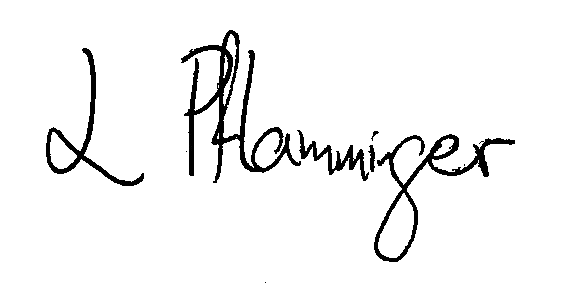
\includegraphics[width=0.35\textwidth]{unterschrift}\vspace*{-0.35cm}
		\\
		\rule[0.5ex]{12em}{0.55pt} & \rule[0.5ex]{12em}{0.55pt} \\
		(Ort, Datum) & (Eigenhändige Unterschrift)
		\\
	\end{tabular*} \\
\end{table}

\newpage


%-----------------------------------
% Seitennummerierung auf arabisch und ab 1 beginnend umstellen
%-----------------------------------
\pagenumbering{arabic}
\setcounter{page}{1}

%-----------------------------------
% Kapitel / Inhalte
%-----------------------------------
% Die Kapitel werden über folgende Datei eingebunden
% Hinzugefügt aufgrund von Issue 167
%-----------------------------------
% Kapitel / Inhalte
%-----------------------------------
% this file is imported into thesis_main.tex
% the section files are not imported directly!

\section{Introduction}
% Could also be Motivation & Problem Definition, Goal and Approach
% Or Motivation and Methodology
\subsection{Abstract}

\subsection{Motivation}

One of the most difficult aspects of operating a website or app is dealing with user
authentication and passwords.

Regularly, hackers try to break into the databases of internet services to reveal account data and 
passwords of their users.

The best-practices for encrypting passwords and storing them safely are changing
continuously and keeping up with new security standards and requirements is costly and time consuming.

Managing passwords and usernames is not only a technical challenge, but also puts a burden
on end users.\footcite[Cp. ][p. 459]{Hoonakker2009}

A majority of users still don't manage their passwords in the recommended way, which is
generating a new password for each login and storing every password in a secure password safe.
A modern internet user on average uses x different services that require a login.
This results in most users using the same password for many or all of these services,
which makes it easy for hackers to overtake a users online presence if only one of their
passwords is hacked or leaked.

Because of these problems, SSO is good fivehead.







Digital services have revolutionized the way people 


Remembering passwords is hard bla bla

Reusing the same password is insecure and hackers have used this



- Account management is hard
- Hackers are trying to find security flaws and publish passwords
- Two factor authentication is annoying for customers etc.



Das Geschäftliche Umfeld moderner Unternehmen ist wechselhaft und komplex.
Kundenanforderungen sowie Marktbedingungen verändern sich stetig und der Hohe Grad an
Vernetzung zwischen verschiedenen Anwendungen erschwert die Übersicht.
Aufgrund dieser schweren Bedingungen, benötigen große Softwareunternehmen wie
Microsoft oder Alphabet Möglichkeiten, schnell auf sich ändernde Bedingungen zu reagieren,
Kundenanforderungen rasant umzusetzen und die Zusammenarbeit und Wissensverteilung effizient
zu organisieren. In dieser Arbeit wird untersucht, ob das Konzept DevOps plausible
Chancen bietet, um diesen hohen Anforderungen gerecht zu werden.

\subsection{Problem Definition and Goal}

Ziel dieser Arbeit ist es, die Prinzipien des DevOps Konzepts im Software Engineering
zu beschreiben, sowie seine Chancen für Unternehmen und Entwicklungsteams darzulegen.
Zudem soll DevSecOps thematisch eingeordnet werden. 

\subsection{Approach}

Die Arbeit beginnt mit einer Darstellung und Erklärung des Software Lebenszyklus und seiner
Schritte. Anschließend wird das Wasserfallmodell als Beispiel für ein konventionelles Ablaufmodell
erläutert. Agile Entwicklung wird abgegrenzt und anhand von Scrum erklärt.
Im Hauptteil wird zunächst der Begriff DevOps definiert und Ursprung und Ziel des Konzepts
erläutert. Anschließend werden die Grundsätze von DevOps anhand der sechs Säulen dargelegt.
Nachdem die Prinzipien von DevOps klar sind, werden Chancen gegeben, die DevOps modernen
Softwareunternehmen bietet. Daraufhin wird der Begriff DevSecOps im Kontext von DevOps eingeordnet.
Abschließend werden die Erkenntnisse zusammengefasst und mögliche Kritik am Konzept adressiert.
\newpage
\section{Fundamentals of Single Sign-On}

% Maybe section about authentication and authorization
\subsection{Basics of Authentication}
\subsubsection{Authentication \& Authorization}
\label{sec:authn_authz}

Authentication is the act of establishing a user's identity. The user has to prove, that they are who they say
they are\footcite[Cp.][p. 398]{Basavala2012}.
There are three main ways how a user can prove their identity:
\begin{enumerate}
    \item The user provides some secret, that only they know, e.g. a password.
    \item The user provides something, that only they have.
          An example for this is a \ac{SMS} based authentication system, where the user receives a message containing a code,
          which has to be entered into the login form. They thus prove, that they are in possession of the phone with the phone
          number they have previously provided.
    \item The user proves their identity by using some unique physical characteristic, e.g. a fingerprint or eye retina scan.\footcite[Cp.][p. 398]{Basavala2012}
\end{enumerate}
Using only one of these ways to authenticate a user is called \ac{SFA}, using two is called \ac{2FA} and using 
multiple factors is called \ac{MFA}.
Using two or more factors for authentication improves security and is deemed essential for applications with sensitive data.\footcite[Cp.][]{Drew2019}

Contrary to authentication, authorization determines whether a user is allowed to access a specific resource.
It happens once the user has been authenticated.\footcite[Cp.][]{Auth0AuthNvsAuthZ} For example, user \emph{A} might make a post on a social media site
which is only shared with their close friends. If user \emph{B} wants to view the post, the system first checks
if user \emph{B} is part of user \emph{A}'s close friends. If they are, they are authorized to see the resource.

\subsubsection{Authentication flows without SSO}

Figure \ref{fig:sfa_flow_chart} shows a flow chart for a traditional authentication flow using a username and password.
The user enters their information and clicks the "Sign In" button. Next, the server checks in a database
whether or not the username exists and if the password is correct. If this is true, the user is authenticated
and is allowed to enter the website.\footcite[Cp.][p. 400]{Basavala2012}

\begin{figure}[H]
    \centering
    \caption{Flow chart of an SFA authentication process}
	\label{fig:sfa_flow_chart}
    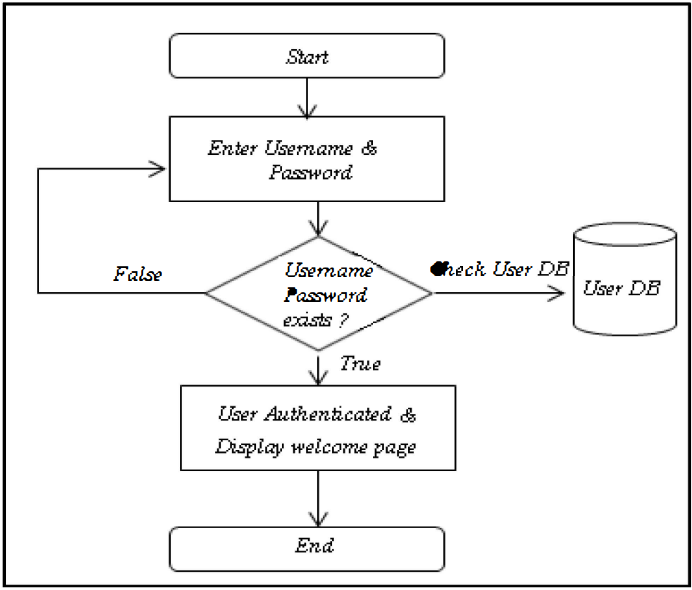
\includegraphics[width=0.5\textwidth]{sfa_flow_chart.png}
    \\
    \cite[Source:][]{Basavala2012}
\end{figure}

Using \ac{2FA} introduces complexity into this process, as the user now has to additionally provide something they have.
In the case of \ac{SMS} \ac{2FA} there are now multiple database tables needed to store passwords,
phone numbers and the codes sent via \ac{SMS}\footcite[Cp.][p. 400]{Basavala2012}. 
Additionally, software needs to be integrated which generates the
codes and sends them to the user.
Managing this complexity and ensuring security for all components is both time- and cost-intensive.

\newpage

\subsection{Single Sign-On and Federated Identity}
\label{sec:sso_fim}
\subsubsection{Definitions}

\ac{SSO} is a mechanism which allows users to sign into multiple independent software systems
using a single set of credentials\footcite[Cp.][134]{Radha2012}.
It also only requires the user to perform a single action to authenticate for multiple participating services.
Such systems or services could be apps, websites or technical interfaces like \acp{API}.
After signing in, the user is not asked to re-enter their password when visiting a different service.\footcite[Cp.][p. 18]{Bazaz2016}

\ac{SSO} is made possible by an \ac{IdP}, which provides a central server for authentication.
When talking about \ac{SSO}, the website operator is usually refered to as the \ac{SP}.
Users authenticate with the \ac{IdP} which shares the user's identity information with the \ac{SP}.\footcite[Cp.][p. 24]{Beltran2016}\footcite[Cp.][p. 25]{Bauer2013}
The \ac{SP} does not confirm the user's identity in any way, so they have to trust the \ac{IdP} to correctly
deliver user identities\footcite[Cp.][]{Nallathamby2018}.
Originally, \ac{SSO} could only be used by members of a single organization to sign into different 
applications like HR software, payroll or communication systems because there were no open standards
that allowed companies to share identities with other organizations.\footcite[Cp.][]{OktaFIM}

\ac{FIM} is the broader term for managing user identities across apps and websites from different organizations and companies.
It provides standards which companies can use to share user identities between trusted domains,
which allows \ac{SSO} to be deployed not just in organizations, but also on the open web.
These standards are what allows end-users to use \acp{IdP} like Google and Facebook to sign into many
different websites.\footcite[Cp.][]{OktaFIM}\footcite[Cp.][p. 1]{Miculan2011}

\subsubsection{Types \& Use Cases of SSO}

Figure \ref{fig:sso_types} shows the different types of \ac{SSO}.
Intranet \ac{SSO} is used within the secure network of an organization and allows its members to 
access multiple applications with one set of credentials. This is relatively easy to deploy, as all components
and clients are administrated by the same organization, eliminating the need for open standards and trust to
third parties.
Extranet \ac{SSO} connects \acp{SP} from different organizations.
This is the basis for Web \ac{SSO} and by extension Social Login, which is the type this paper is mainly concerned with.
It is based on web technologies and allows users to access different public websites with a single set of credentials.\footcite[Cp.][p. 135]{Radha2012}

\begin{figure}[H]
    \centering
    \caption{Types of Single Sign-On}
	\label{fig:sso_types}
    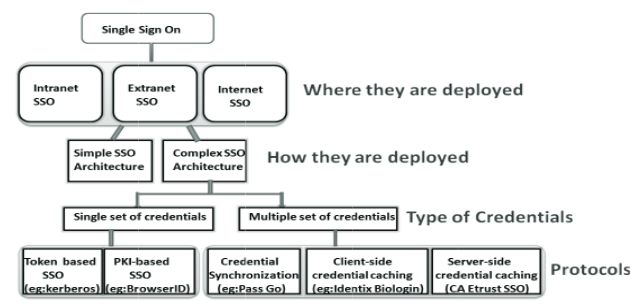
\includegraphics[width=0.8\textwidth]{sso_types.png}
    \\
    \cite[Source:][]{Radha2012}
\end{figure}

\subsubsection{Web SSO Protocols \& Technologies}

There are many different protocols defined for \ac{SSO}.
Some are only used for Intranet \ac{SSO}, which is not covered in this paper.
The next section only covers the three most used Web \ac{SSO} protocols\footcite[Cp.][]{OneLoginFIMTechnologies}.

\textbf{Security Assertion Markup Language}

\ac{SAML} is an open standard for exchanging user identities and authorization information between
an \ac{IdP} and an \ac{SP}\footcite[Cp.][p. 1]{Gross}.
It uses the \ac{XML} for communication between applications.
The typical authentication flow using \ac{SAML} is shown in figure \ref{fig:flow_saml}.
An \ac{SP} contacts an \ac{IdP} and requests a user identity.
The \ac{SAML} standard does not specify how the \ac{IdP} has to authenticate the user,
but only defines the communication between the two parties.
After the user has authenticated with the \ac{IdP}, the identity information is sent back to 
the \ac{SP}. It includes, whether the user is authenticated, what roles and rights they have and
which data and resources they are allowed to access.\footcite[Cp.][p. 137]{Radha2012}
Note that, while the \ac{SP} basically communicates directly with the \ac{IdP}, all communication
still goes through the user's client. Which \ac{IdP} is used is predefined by the \ac{SP}. The user does not
get to choose, where they enter their credentials or who provides their identity.\footcite[Cp.][p. 21]{Bazaz2016}
The \ac{SP} has to trust the \ac{IdP} completely, because it also handles authorization. 

\begin{figure}[H]
    \centering
    \caption{Flow of SAML Protocol}
	\label{fig:flow_saml}
    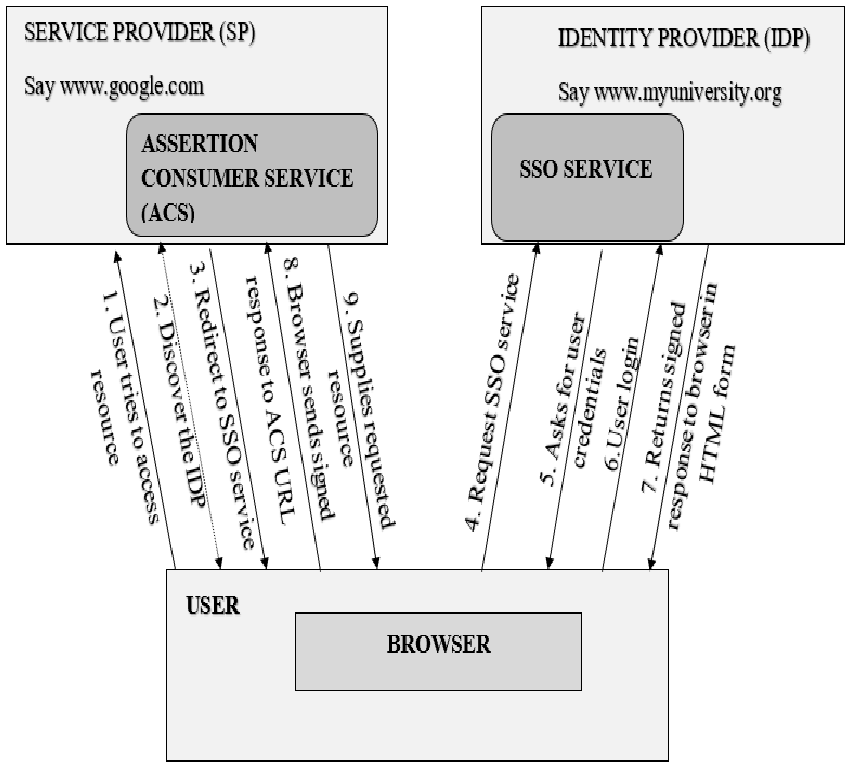
\includegraphics[width=0.5\textwidth]{flow_saml.png}
    \\
    \cite[Source:][p. 21]{Bazaz2016}
\end{figure}

\textbf{OpenID}

This protocol works differently than \ac{SAML}, in that the user gets to choose who provides their identity.
They might use a large \ac{IdP} like Google or Facebook or even set up their own OpenID service.
The \ac{SP} is called the \ac{RP} in this model. The \ac{IdP} is only responsible for authentication of users
and providing identity. It does not deliver any authorization information.\footcite[Cp.][p. 21]{Bazaz2016}
The flow is shown in figure \ref{fig:flow_openid}.

The user visits the website and clicks the sign in button. They are then prompted to enter their OpenID \ac{IdP}.
The \ac{RP} (the website) then redirects the user to the site of the \ac{IdP}, where the user authenticates by
entering their credentials. In the next step the user tells the \ac{IdP} which information they want to share with
the \ac{RP}. If the credentials are valid, the selected identity information is passed to the \ac{RP}, otherwise
the user is asked to enter valid credentials.\footcite[Cp.][p. 21]{Bazaz2016}
This seperation of \ac{RP} and \ac{IdP} and introduction of user choice is the basis for Web \ac{SSO} as it is used today,
where websites allow users to choose their preferred identity provider.
\ac{SAML} does not allow for this, as the \ac{IdP} is predefined by the \ac{SP}.

\begin{figure}[H]
    \centering
    \caption{Flow of OpenID Protocol}
	\label{fig:flow_openid}
    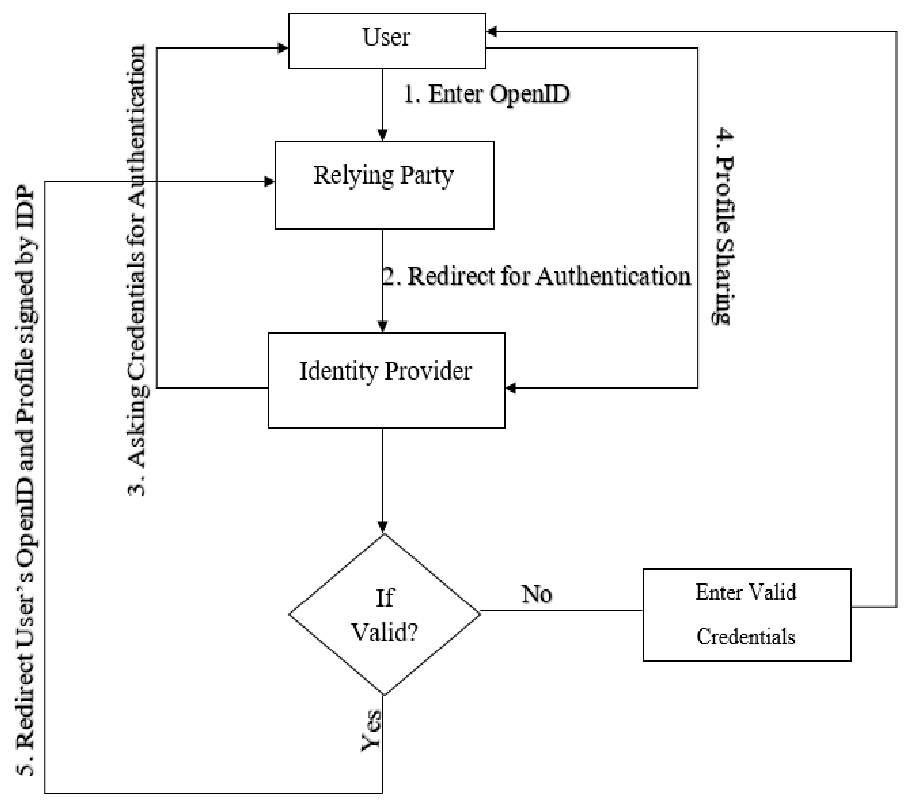
\includegraphics[width=0.5\textwidth]{flow_openid.png}
    \\
    \cite[Source:][p. 22]{Bazaz2016}
\end{figure}

\textbf{OAuth 2.0 \& OpenID Connect}

OAuth 2.0 differentiates from the other protocols, in that it centers around authorization rather than authentication.
An example use case for this is a third-party app wanting to create a Facebook post in the user's name on their profile (see figure \ref{fig:flow_oauth2}).
For this, the app does not need an identity, but rather Facebook's permission to create a post.
It contacts Facebook's OAuth Server and asks it for permission. Facebook then contacts the user which owns the resource
(in this case the Facebook account) and asks them for permission. They accept by logging into their account and accepting
access from the app. The Facebook OAuth Server sends back a token to the app which can be used to create the post.
The app then contacts Facebook's resource server to actually create the post, providing the token to prove it is authorized.\footcite[Cp.][]{Wesener2021}

\begin{figure}[H]
    \centering
    \caption{Flow of OAuth 2.0 Protocol}
	\label{fig:flow_oauth2}
    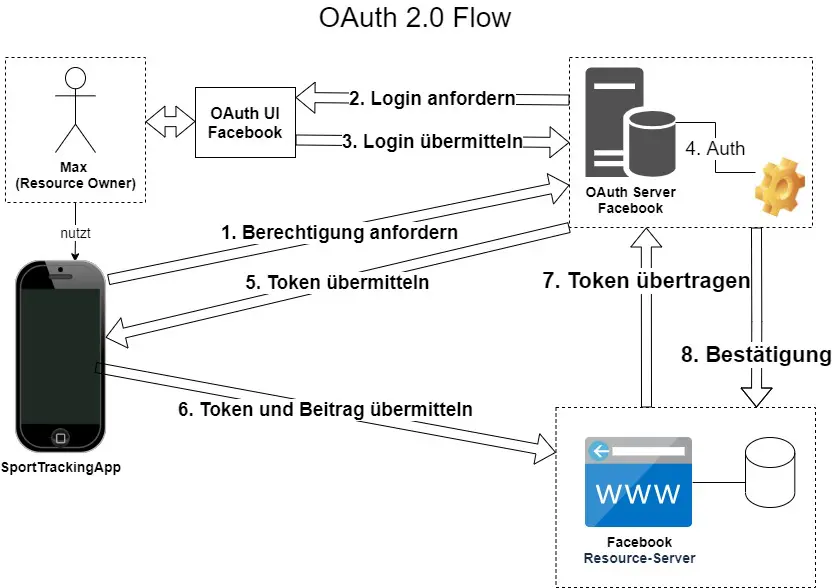
\includegraphics[width=0.8\textwidth]{flow_oauth2.png}
    \\
    \cite[Source:][p. 22]{Wesener2021}
\end{figure}

While OAuth 2.0 is a protocol specification, OpenID Connect is a concrete implementation of the protocol\footcite[Cp.][p. 189]{Fett2017}.
It also provides a way to do authentication via the OAuth 2.0 protocol, even though it was not designed for that\footcite[Cp.][]{Hrnjadovic2020}.
The terms "OpenID" and "OpenID Connect" are different and can't be used interchangeably.\footcite[Cp.][]{Wesener2021}

To further understand the difference between the OAuth 2.0 and OpenID functionalities consider an e-commerce example,
where the user has to enter their payment information. They have previously entered it into their Google account and would
like to automatically fill the information from Google into the shop's form.

Using OpenID, the shop would use Google as an \ac{IdP} to get the user's identity and automatically create a corresponding
user account on the website. As OpenID simply provides the identity and can't retrieve the payment information from Google,
the user would still have to enter their payment information manually.
It would then be saved in the user's account on the web shop (not Google) and when they return to buy a different item,
the information could be retrieved from the \ac{SP}'s server.

With OAuth, the \ac{SP} would not have to create a user account using the identity from Google and would not have to store any
information on its server. It would simply request access to the payment information resource from Google. The user would
authenticate and allow the information transfer. Then, the \ac{SP} could retrieve the information from Google and use it
in the checkout process.

\subsection{Web SSO Providers}

\subsubsection{Overview}

There are many \ac{SSO} solutions targeted at businesses for internal use.
In addition to an \ac{IdP} service they often provide an identity management suite which allows businesses
to easily deploy \ac{SSO} within their network.\footcite[Cp.][]{Witts2022}
The solutions targeting end users on the open web are often called "Social Login" services, as they rely on 
social networks that have a large userbase like Facebook, Twitter, Google or LinkedIn.\footcite[Cp.][p. 2]{Gafni2014}

The most popular social networks worldwide are Facebook with 2.9 billion and YouTube with 2.6 billion monthly 
active users\footcite[Cp.][]{StatistaSocial2022}.
As YouTube is based on user accounts from Google, their social login offering is examined here.

\subsubsection{Sign In With Google}
\label{sec:sign_in_with_google}

Google's service is based on the OAuth 2.0 protocol. This ensures a flexible service,
as \acp{SP} can create a seperate account on their server, but do not have to, as they can retrieve
required resources using OAuth.\footcite[Cp.][]{GoogleSignIn2022}
Customizable buttons are provided by Google, which redirect the user to Google's sign in page (figure \ref{fig:google_sign_in_ui}a).
Google claims data from the feature is not used for advertising or other non-related purposes.
If users are already signed into their Google account when visiting the website, Google offers the
possibility to sign in with one click using a pop up, as shown in figure \ref{fig:google_sign_in_ui}b.
Google offers an additional autorization interface to allow loading other data from a users Google account.\footcite[Cp.][]{GoogleSignIn2022}

\begin{figure}[H]
    \caption{Sign In With Google UI}%
    \centering
    \subfloat[Sign In With Google Button]{{
\includegraphics[width=0.2\textwidth]{google_sign_in_button.png}}}%
    \hfill
    \subfloat[One-Tap Sign In]{{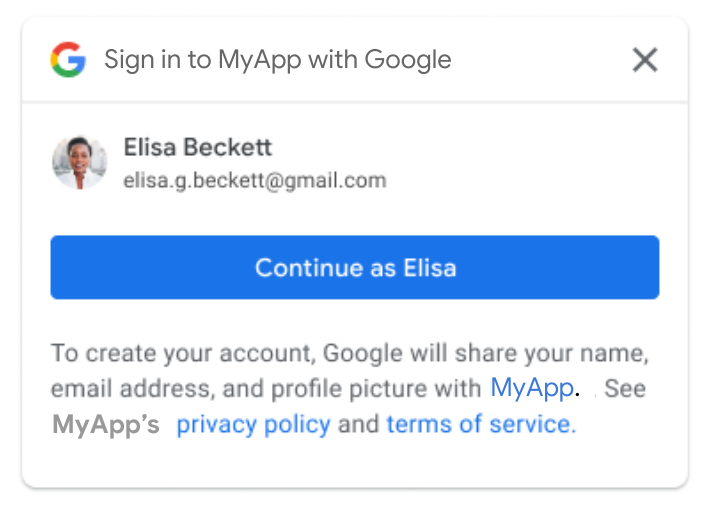
\includegraphics[width=0.3\textwidth]{google_one_tap.png}}}%
    \hfill
    \subfloat[Google Password Prompt]{{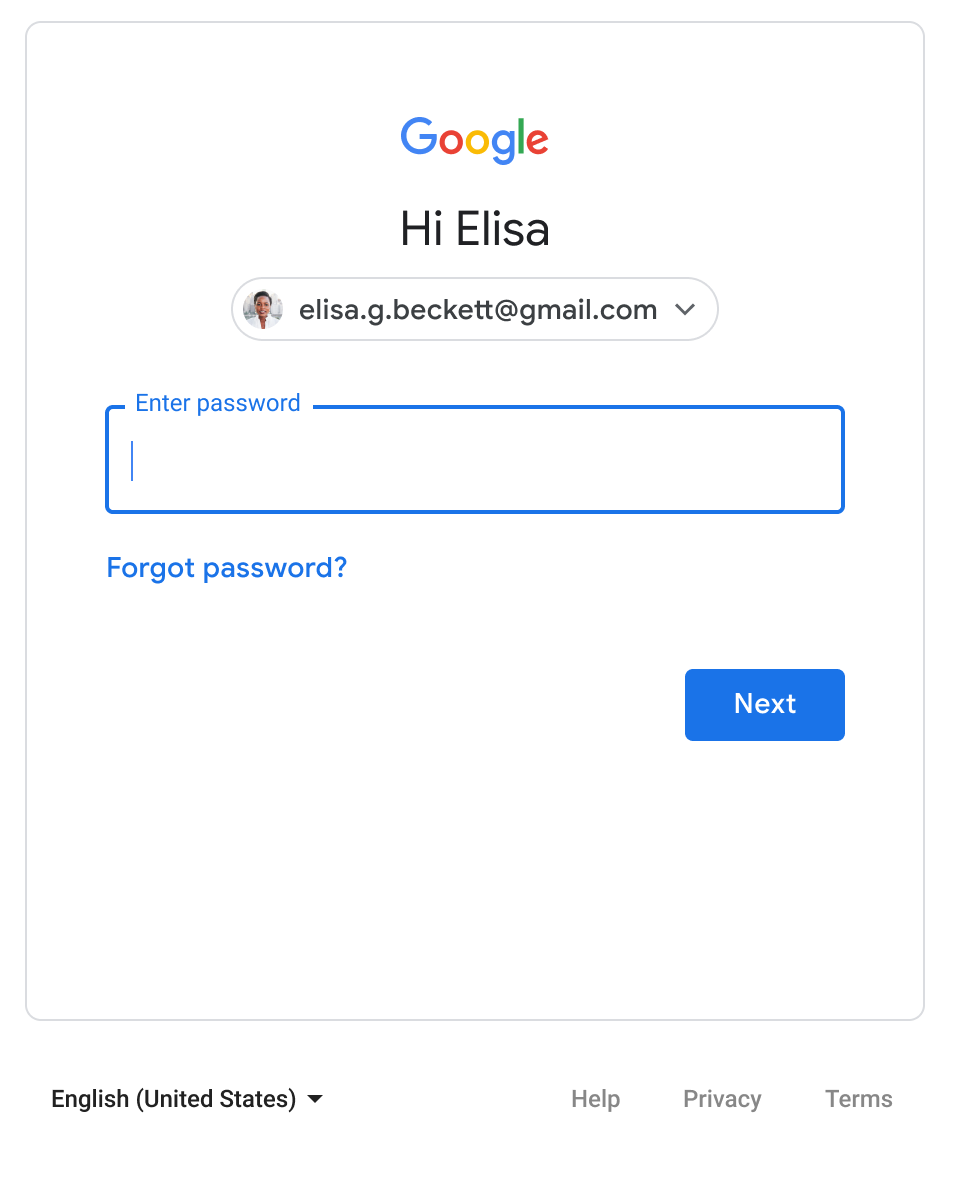
\includegraphics[width=0.4\textwidth]{google_password_prompt.png}}}%
    \\
    \cite[Source:][]{GoogleSignIn2022}
    \label{fig:google_sign_in_ui}%
\end{figure}

Integrating the Sign In With Google service into an existing website is fairly easy.
\acp{SP} have to create a project on Google's developer website. They then have the option
to configure the consent screen shown to the user by Google and enter information like their website name and logo,
a support e-mail address and which user data the application wants to retrieve.\footcite[Cp.][]{GoogleSignIn2022}

Website developers can integrate Google's authentication interface into the website with just a few lines of code.
After the user authenticates, the user data is delivered into the web application and can be used from there.
If \acp{SP} have existing account management infrastructure, integrating this method might certainly require
more time, as data might come in a different format or database structures might not line up.\footcite[Cp.][]{GoogleSignIn2022}
\newpage
\section{Opportunities}

\subsection{Higher Conversion Rates}

\subsection{Simpler Account Management}
%Only using SSO providers and thus not having to store passwords...

\subsection{Lower Risk of Data Leaks}

\subsection{Cross-Platform User Tracking}
\newpage

\section{Risks of using \ac{SSO} Services}

\subsection{Association with providers}

\subsection{Loss of Users}

\subsection{Leakage of User Data}

\subsection{Technical Complexity of Integration}
\section{Conclusion}


%-----------------------------------
% Apendix / Anhang
%-----------------------------------
%\newpage
%\section*{\AppendixName} %Überschrift "Anhang", ohne Nummerierung
%\addcontentsline{toc}{section}{\AppendixName} %Den Anhang ohne Nummer zum Inhaltsverzeichnis hinzufügen
%
%\begin{appendices}
%% Nachfolgende Änderungen erfolgten aufgrund von Issue 163
%\makeatletter
%\renewcommand\@seccntformat[1]{\csname the#1\endcsname:\quad}
%\makeatother
%\addtocontents{toc}{\protect\setcounter{tocdepth}{0}} %
%	\renewcommand{\thesection}{\AppendixName\ \arabic{section}}
%	\renewcommand\thesubsection{\AppendixName\ \arabic{section}.\arabic{subsection}}
%	\input{sections/06_Anhang/anhang}
%\end{appendices}
%\addtocontents{toc}{\protect\setcounter{tocdepth}{2}}

%-----------------------------------
% Literaturverzeichnis
%-----------------------------------
\newpage

% Die folgende Zeile trägt ALLE Werke aus literatur.bib in das
% Literaturverzeichnis ein, egal ob sie zietiert wurden oder nicht.
% Der Befehl ist also nur zum Test der Skripte sinnvoll und muss bei echten
% Arbeiten entfernt werden.
%\nocite{*}

%\addcontentsline{toc}{section}{Literatur}

% Die folgenden beiden Befehle würden ab dem Literaturverzeichnis wieder eine
% römische Seitennummerierung nutzen.
% Das ist nach dem Leitfaden nicht zu tun. Dort steht nur dass 'sämtliche
% Verzeichnisse VOR dem Textteil' römisch zu nummerieren sind. (vgl. S. 3)
%\pagenumbering{Roman} %Zähler wieder römisch ausgeben
%\setcounter{page}{4}  %Zähler manuell hochsetzen

% Ausgabe des Literaturverzeichnisses

% Keine Trennung der Werke im Literaturverzeichnis nach ihrer Art
% (Online/nicht-Online)
%\begin{RaggedRight}
%\printbibliography
%\end{RaggedRight}

% Alternative Darstellung, die laut Leitfaden genutzt werden sollte.
% Dazu die Zeilen auskommentieren und folgenden code verwenden:

% Literaturverzeichnis getrennt nach Nicht-Online-Werken und Online-Werken
% (Internetquellen).
% Die Option nottype=online nimmt alles, was kein Online-Werk ist.
% Die Option heading=bibintoc sorgt dafür, dass das Literaturverzeichnis im
% Inhaltsverzeichnis steht.
% Es ist übrigens auch möglich mehrere type- bzw. nottype-Optionen anzugeben, um
% noch weitere Arten von Zusammenfassungen eines Literaturverzeichnisse zu
% erzeugen.
% Beispiel: [type=book,type=article]
\printbibliography[nottype=online,heading=bibintoc,title={\langde{Literaturverzeichnis}\langen{Bibliography}}]

% neue Seite für Internetquellen-Verzeichnis
\newpage

% Laut Leitfaden 2018, S. 14, Fussnote 44 stehen die Internetquellen NICHT im
% Inhaltsverzeichnis, sondern gehören zum Literaturverzeichnis.
% Die Option heading=bibintoc würde die Internetquelle als eigenen Eintrag im
% Inhaltsverzeicnis anzeigen.
\printbibliography[type=online,heading=bibintoc,title={\headingNameInternetSources}]
%\printbibliography[type=online,heading=subbibliography,title={\headingNameInternetSources}]

\newpage
\pagenumbering{gobble} % Keine Seitenzahlen mehr

%-----------------------------------
% Ehrenwörtliche Erklärung
%-----------------------------------
\section*{%
	\langde{Ehrenwörtliche Erklärung}
	\langen{Declaration in lieu of oath}}
\langde{Hiermit versichere ich, dass die vorliegende Arbeit von mir selbstständig und ohne unerlaubte Hilfe angefertigt worden ist, insbesondere dass ich alle Stellen, die wörtlich oder annähernd wörtlich aus Veröffentlichungen entnommen sind, durch Zitate als solche gekennzeichnet habe. Ich versichere auch, dass die von mir eingereichte schriftliche Version mit der digitalen Version übereinstimmt. Weiterhin erkläre ich, dass die Arbeit in gleicher oder ähnlicher Form noch keiner Prüfungsbehörde/Prüfungsstelle vorgelegen hat. Ich erkläre mich damit einverstanden, dass die Arbeit der Öffentlichkeit zugänglich gemacht wird. Ich erkläre mich damit einverstanden, dass die Digitalversion dieser Arbeit zwecks Plagiatsprüfung auf die Server externer Anbieter hochgeladen werden darf. Die Plagiatsprüfung stellt keine Zurverfügungstellung für die Öffentlichkeit dar.}
\langen{I hereby declare that I produced the submitted paper with no assistance from any other party and without the use of any unauthorized aids and, in particular, that I have marked as quotations all passages which are reproduced verbatim or near-verbatim from publications. Also, I declare that this paper has never been submitted before to any examination board in either its present form or in any other similar version. I herewith agree that this paper may be published. I herewith consent that this paper may be uploaded to the server of external contractors for the purpose of submitting it to the contractors' plagiarism detection systems. Uploading this paper for the purpose of submitting it to plagiarism detection systems is not a form of publication.}


\par\medskip
\par\medskip

\vspace{5cm}

\begin{table}[H]
	\centering
	\begin{tabular*}{\textwidth}{c @{\extracolsep{\fill}} ccccc}
		\myOrt, \the\day.\the\month.\the\year
		&
		% Hinterlege deine eingescannte Unterschrift im Verzeichnis /abbildungen und nenne sie unterschrift.png
		% Bilder mit transparentem Hintergrund können teils zu Problemen führen
		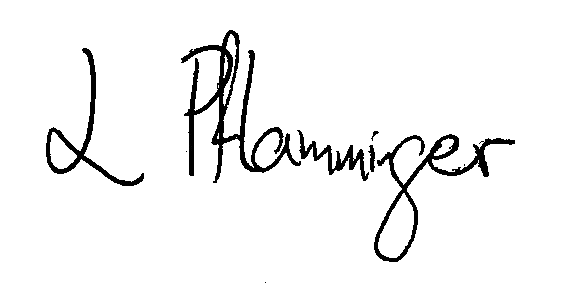
\includegraphics[width=0.35\textwidth]{unterschrift}\vspace*{-0.35cm}
		\\
		\rule[0.5ex]{12em}{0.55pt} & \rule[0.5ex]{12em}{0.55pt} \\
		\langde{(Ort, Datum)}\langen{(Location, Date)} & \langde{(Eigenhändige Unterschrift)}\langen{(handwritten signature)}
		\\
	\end{tabular*} \\
\end{table}

\end{document}
